\documentclass[t]{sdqbeamer}
%\documentclass[c]{sdqbeamer} 

\usepackage{listings}
\usepackage{graphicx}
\usepackage{tabularx}
\usepackage{tikzsymbols}
\usepackage{tikz}
\usetikzlibrary{positioning,fit,shapes}
\usepackage[lined,linesnumbered,ruled,noend]{algorithm2e}

\hypersetup{
	colorlinks=true,
	urlcolor=kit-orange
}

% set sdqbeamer options
\titleimage{blender-render}
\groupname{Algorithm Engineering}
\grouplogo{ae}
\selectlanguage{english}

% define title etc.pp.
\title[SAT Solving]{Practical SAT Solving}
\subtitle{Lecture 4}
\author{\underline{Markus Iser}, Dominik Schreiber, Tom\'a\v{s} Balyo}
\date{May 06, 2024}

% Existing KIT colors: kit-green, kit-blue, kit-red, kit-gray, kit-orange, kit-lightgreen, kit-brown, kit-purple, kit-cyan
% configure appearance
\setbeamercolor{block title}{bg=kit-blue}
\setbeamercolor{block body}{bg=kit-blue!10}
\setbeamercolor{block title example}{bg=kit-orange}
\setbeamercolor{block body example}{bg=kit-orange!10}
\setbeamertemplate{itemize item}{\color{kit-gray}\textbullet}
\setbeamertemplate{itemize subitem}{\color{kit-gray}\textbullet}
\setbeamercolor{item projected}{bg=kit-gray, fg=kit-gray}
\renewcommand{\insertnavigation}[1]{} % remove navigation bar

% define commands
\definecolor{myblue}{HTML}{0D3B66}
\definecolor{myred}{HTML}{6E0E0A}
\definecolor{mypink}{HTML}{F7B2B7}

\newcommand{\vars}[1]{\textsf{vars} (#1)}
\newcommand{\lits}[1]{\textsf{lits} (#1)}
\newcommand{\clss}[1]{\textsf{clss} (#1)}

\newcommand{\highl}[1]{\textcolor{myblue}{#1}}
\newcommand{\highlo}[1]{\textcolor{myred}{#1}}
\newcommand{\highlow}[1]{\textcolor{mypink}{#1}}

% Extra column types for tabularx
\newcolumntype{C}{>{\centering\arraybackslash}X}
\newcolumntype{L}{>{\raggedright\arraybackslash}X}
\newcolumntype{R}{>{\raggedleft\arraybackslash}X}

\newcommand{\setcolsep}[1]{\setlength{\tabcolsep}{#1}}
\newcommand{\setrowsep}[1]{\renewcommand{\arraystretch}{#1}}

% Definitions for the Tseitin transformation
\newcommand{\true}{\ensuremath{\mathit{True}}}
\newcommand{\false}{\ensuremath{\mathit{False}}}
\newcommand{\allvars}{\ensuremath{\mathcal{V}}}
\newcommand{\tseitin}[1]{\ensuremath{\mathcal{T}(#1)}}
\newcommand{\tseitinRec}[2]{\ensuremath{\mathcal{T}^{#2}(#1)}}
\newcommand{\tseitinSym}[1]{\ensuremath{\mathcal{T}_\mathsf{lit}(#1)}}
\newcommand{\tseitinDef}[2]{\ensuremath{\mathcal{T}_\mathsf{def}^{#2}(#1)}}
\newcommand{\hcancel}[2][black]{\setbox0=\hbox{$#2$}\rlap{\raisebox{.45\ht0}{\textcolor{#1}{\rule{\wd0}{1pt}}}}#2} 
\newcommand{\sateq}{\mathrel{\overset{\makebox[0pt]{\mbox{\normalfont\tiny\sffamily SAT}}}{=}}}

\newcommand{\enc}{\ensuremath{\mathcal{E}}} % encoding

% exercise commands
\newcommand{\exhead}[3]{
\hrule~\\[1ex]\noindent
{\bf Practical SAT Solving} (ST 2024) \hfill \fbox{Assignment #1} \\[1ex]
Markus Iser, Dominik Schreiber, Tom\'a\v{s} Balyo\\[1ex]
Algorithm Engineering (KIT) \hfill #2 -- #3\\
\hrule
\thispagestyle{empty}
}
\setlength{\itemsep}{1em}

\begin{document}

\begin{frame}
	\thispagestyle{empty}
	\titlepage
\end{frame}

\begin{frame}{Overview}
	\begin{block}{Recap. Lecture 3: Classic Algorithms}
		\begin{itemize}\setlength{\itemsep}{1ex}
			\item Local Search
			\item Resolution
			\item DP Algorithm
			\item DPLL Algorithm
		\end{itemize}
	\end{block}
	\pause
	\begin{block}{Today's Topics}
		\begin{itemize}\setlength{\itemsep}{1ex}
			\item Classic Heuristics: Branching Order, Branching Polarity, Restart Strategies
			\item Modern SAT Solving 1: Conflict Analysis, Clause Learning
		\end{itemize}
	\end{block}
\end{frame}

\begin{frame}{DPLL Algorithm: Iterative Variant}\begin{block}{}
\begin{columns}[T]
\begin{column}{.3\linewidth}
~\\[1em]
\textbf{Decision Heuristics:}~\\[1em]
\begin{itemize}\setlength{\itemsep}{1em}
	\item Branching Order:\\[1ex] Which variable to choose?
	\item Branching Polarity:\\[1ex] Which value to assign?
\end{itemize}
\end{column}
\begin{column}{.6\linewidth}
\begin{algorithm}[H]
\DontPrintSemicolon
\caption{iterativeDPLL(CNF Formula $F$)}
\KwData{Trail (Stack of Literals)}
\BlankLine

\While{not all variables assigned by Trail} {
	\If{unitPropagation(F, Trail) has CONFLICT} {
		$L \leftarrow$ last literal not tried both True and False\;
		\lIf {no such $L$} {\Return UNSAT}
		pop all literals after and including $L$ from Trail\;
		push $\{ L = 0 \}$ on Trail\;
	}
	\Else{ 
		\highlo{$L \leftarrow$ pick an unassigned literal}\;
		push $\{ L = 1 \}$ on Trail \;
	}
}
\Return SAT\;
\end{algorithm}
\end{column}
\end{columns}
\end{block}
\end{frame}

\begin{frame}{Decision Heuristics}
\begin{block}{Properties of Decision Heuristics}
	\begin{itemize}\setlength{\itemsep}{1em}
		\item Desired properties:
		\begin{itemize}\setlength{\itemsep}{1ex}
			\item Fast to compute
			\item Yields easy sub-problems\\
			$\rightarrow$ Maximize unit propagations
		\end{itemize}
		\item Static vs. dynamic:
		\begin{itemize}\setlength{\itemsep}{1ex}
			\item Static: Based on formula statistics
			\item Dynamic: Based on formula and current state
		\end{itemize}
		\item Separate vs. joint:
		\begin{itemize}\setlength{\itemsep}{1ex}
			\item Separate: Choose variable and value independently
			\item Joint: Choose variable and value together
		\end{itemize}
	\end{itemize}
\end{block}
\end{frame}

\begin{frame}{Decision Heuristics: Böhm's Heuristic}
\begin{itemize}\setlength{\itemsep}{1ex}
	\item $h_i(x)$: number of clauses of size $i$ containing literal $x$ which are \highl{not yet satisfied}
	\item $H_i(x) := \alpha \operatorname{max}(h_i(x), h_i(\overline{x})) + \beta \operatorname{min}(h_i(x), h_i(\overline{x}))$ \quad (let $\alpha:=1$ and $\beta:=2$, for example)
	\item Select literal $x$ with the \highl{maximal vector $(H_1(x),H_2(x),\dots)$} under lexicographic order
\end{itemize}
\begin{block}{Properties of Böhm's Heuristic}
Goal: \highl{satisfy or reduce size} of many and preferably short clauses\\[1ex]
\begin{itemize}\setlength{\itemsep}{1em}
	\item Separate polarity heuristic (note that $H_i(x) = H_i(\overline x)$)\\[1ex]
		$\rightarrow$ select $x$ if $\sum_i h_i(x) \geq \sum_i h_i(\overline x)$
	\item depends on literal occurrence counts over the not yet satisfied clauses
	\item \href{https://stamm-wilbrandt.de/en/Report_on_a_SAT_competition.pdf}{SAT Competition 1992:} best heuristic for random instances
\end{itemize}
\end{block}
\end{frame}
	
\begin{frame}{Decision Heuristics: Mom's Heuristic}{\textbf{M}aximum \textbf{O}ccurrences in clauses of \textbf{M}inimum \textbf{S}ize}
\begin{itemize}\setlength{\itemsep}{1ex}
	\item $f^*(x)$: how often $x$ occurs in the \highl{smallest not yet satisfied} clauses
	\item Select variable $x$ with a maximum $S(x) = \bigl(f^*(x)+f^*(\overline{x})\bigr) \cdot 2^k + f^*(x) \cdot f^*(\overline{x})$ \quad (let $k:=10$, for example)
\end{itemize}
\begin{block}{Properties of Mom's Heuristic}
Goal: assign variables with \highl{high occurrence in short clauses}\\[1ex]
\begin{itemize}\setlength{\itemsep}{1em}
	\item Separate polarity heuristic\\[1ex]
		$\rightarrow$ for example, select $x$ if $f^*(\overline x) \geq f^*(x)$
	\item depends on literal occurrence counts over the not yet satisfied clauses
	\item Popular in the mid 90s (Find some variants in \href{https://satlecture.github.io/kit2024/references/1995_Freeman_Thesis.ps}{Freeman 1995})
\end{itemize}
\end{block}
\end{frame}
	
\begin{frame}{Decision Heuristics: Jeroslow-Wang Heuristic}
\begin{itemize}\setlength{\itemsep}{1ex}
	\item Choose the literal $x$ with a maximum $J(x) = \sum_{x \in c,\ c \in F} 2^{-|c|}$
\end{itemize}
\begin{block}{Properties of Jeroslow-Wang Heuristic}
	Goal: assign variables with \highl{high occurrence in short clauses}\\[1ex]
	\begin{itemize}\setlength{\itemsep}{1em}
		\item Considers \highl{all clauses}, but shorter clauses are more important
		\item Separate polarity heuristic\\
		$\rightarrow$ for example, use conflict-seeking polarity heuristic
		\item \highl{Two-sided variant}: choose variable $x$ with maximum $J(x)+J(\overline{x})$\\
		$\rightarrow$ one-sided version works better
	\item Much better experimental results than B{\"o}hm and MOMS
\end{itemize}
\end{block}
\end{frame}
	
\begin{frame}{(R)DLCS and (R)DLIS Heuristics}{(\textbf{R}andomized) \textbf{D}ynamic \textbf{L}argest (\textbf{C}ombined | \textbf{I}ndividual) \textbf{S}um}
\begin{itemize}\setlength{\itemsep}{1ex}
	\item based on positive $C_P(x)$ and negative occurences $C_N(x)$ of variable $x$
	\item used in the famous SAT solver \highl{GRASP} in 2000
\end{itemize}
\begin{block}{Properties of (R)DLCS and (R)DLIS Heuristics}
\begin{itemize}\setlength{\itemsep}{1em}
	\item \highl{Dynamic}: Take the \highl{current partial assignment} into account
	\item \highl{Combined}: select $x$ with maximal $C_P(x)+C_N(x)$
	\item \highl{Individual}: select $x$ with maximal $\operatorname{max}(C_P(x),C_N(x))$
	\item \highl{Randomized}: randomly select variable among the best
\end{itemize}
\end{block}
\end{frame}
	
\iffalse
\begin{frame}{LEFV Heuristic}
\textbf{L}ast \textbf{E}ncountered \textbf{F}ree \textbf{V}ariable:
\begin{itemize}
	\item During unit propagation save the \highl{last unassigned variable} you see
	\item If the variable is \highl{still unassigned} at decision time, use it; \\
	otherwise, choose a \highl{random variable}
	\item \highl{Very fast computation}: constant memory and time overhead
	\begin{itemize}
	\item Requires 1 int variable (to store the last seen unassigned variable)
	\end{itemize}
	\item Maintains \highl{search locality}
	\item Works well for \highlo{Pigeon Hole} and similar formulas
\end{itemize}
\end{frame}
\fi

\begin{frame}{Recap}
\begin{block}{Decision Heuristics}
\begin{itemize}\setlength{\itemsep}{1ex}
	\item Böhm's Heuristic
	\item Mom's Heuristic
	\item Jeroslow-Wang Heuristic
	\item (R)DLCS and (R)DLIS Heuristics
\end{itemize}
\end{block}
\begin{block}{Next up}
	Restart Strategies
\end{block}
\end{frame}
		
\begin{frame}{Restarts Strategies: Motivation}
Given $n$ runs of \highl{randomized DPLL search}, what is the \highl{average number of backtracks} per run (relative to $n$)?
\begin{block}{Heavy-tailed Distribution}
\begin{minipage}{0.5\textwidth}
	\centering
		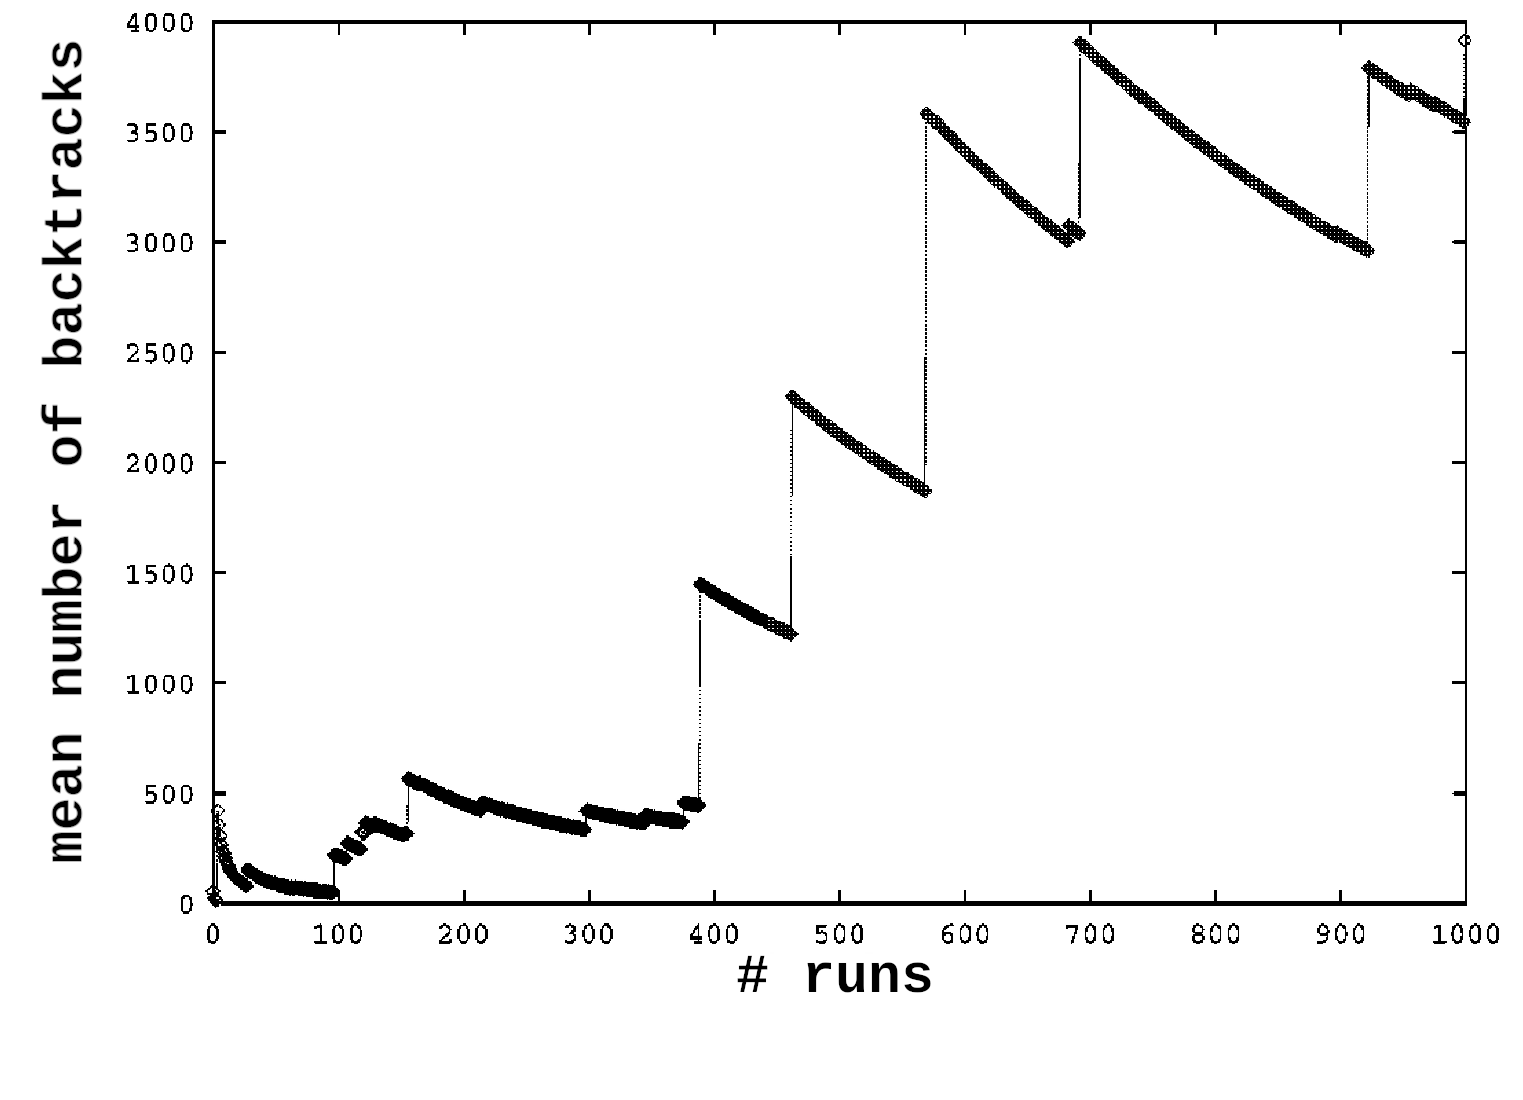
\includegraphics[width=.7\textwidth]{figures/l04/heavy-tail-1}\\
		\highlo{$\Rightarrow$ Heavy-tailed distribution}:
		$P[X > x] \sim C \cdot x^{-\alpha}, \quad C > 0, \alpha \in (0,2)$
\end{minipage}%
\begin{minipage}{0.5\textwidth}
	\centering
	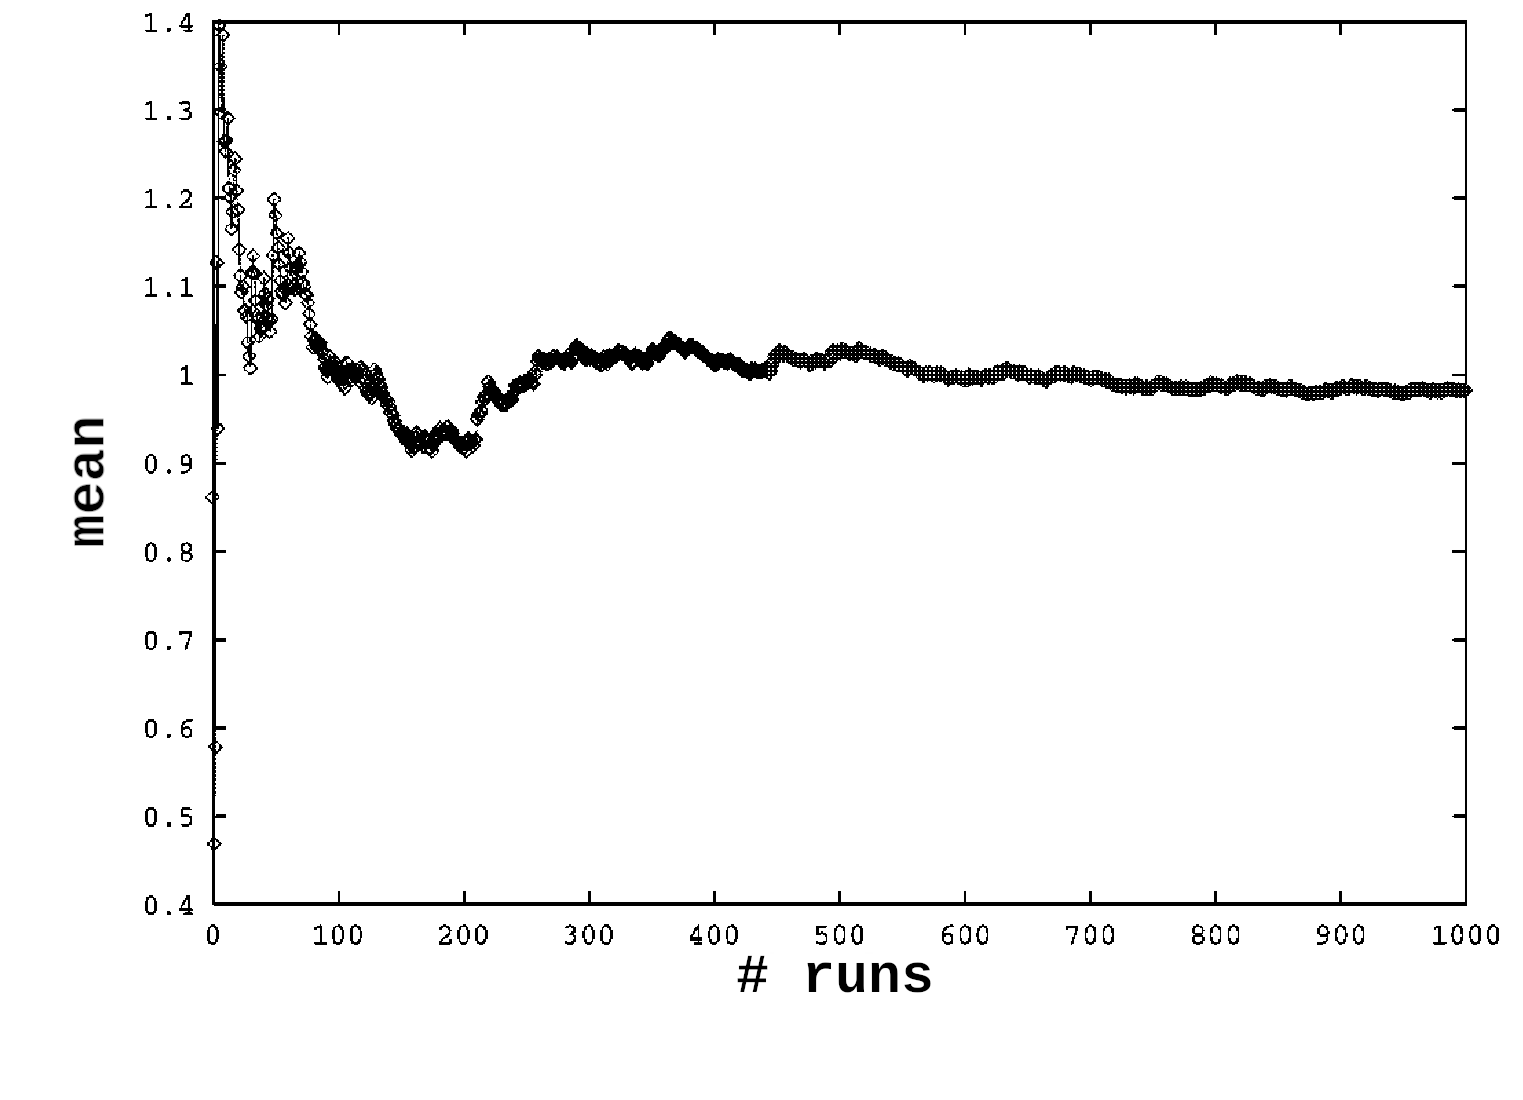
\includegraphics[width=.7\textwidth]{figures/l04/heavy-tail-2}\\
	--- vs. Standard distribution: 
	$P[X > x] \sim \frac{1}{x\sqrt{2\pi}}e^{-x^2/2}$\\[1ex]
	\hfill\small\textcolor{gray}{[From: Gomes et al. 2000]}
\end{minipage}
\end{block}
\end{frame}

\begin{frame}{Restart Strategies}
Clear the partial assignment and backtrack to the root of the search tree.
\begin{block}{Why Restart?}
\begin{itemize}\setlength{\itemsep}{1ex}
	\item To recover from \highlo{bad branching decisions} and solve more instances
	\item Might decrease performance on \highl{easy instances}
\end{itemize}
\end{block}
\begin{block}{When to Restart?}
\begin{itemize}\setlength{\itemsep}{1ex}
	\item After \highl{some number of conflicts / backtracks}
	\item The intervals between restarts should increase \highl{to guarantee completeness}
	\item How much increase?
	\begin{itemize}\setlength{\itemsep}{1ex}
		\item Linear increase -- too slow
		\item Exponential increase -- ok with small exponent
		\item MiniSat: $k$-th restart happens after $100 \times 1.1^k$ conflicts
	\end{itemize}
\end{itemize}
\end{block}
\end{frame}

\begin{frame}{Restart Strategies: Inner / Outer Pattern}
\begin{block}{Inner / Outer Pattern (MiniSat)}
\begin{columns}[T]
\begin{column}{0.5\textwidth}
	\centering
	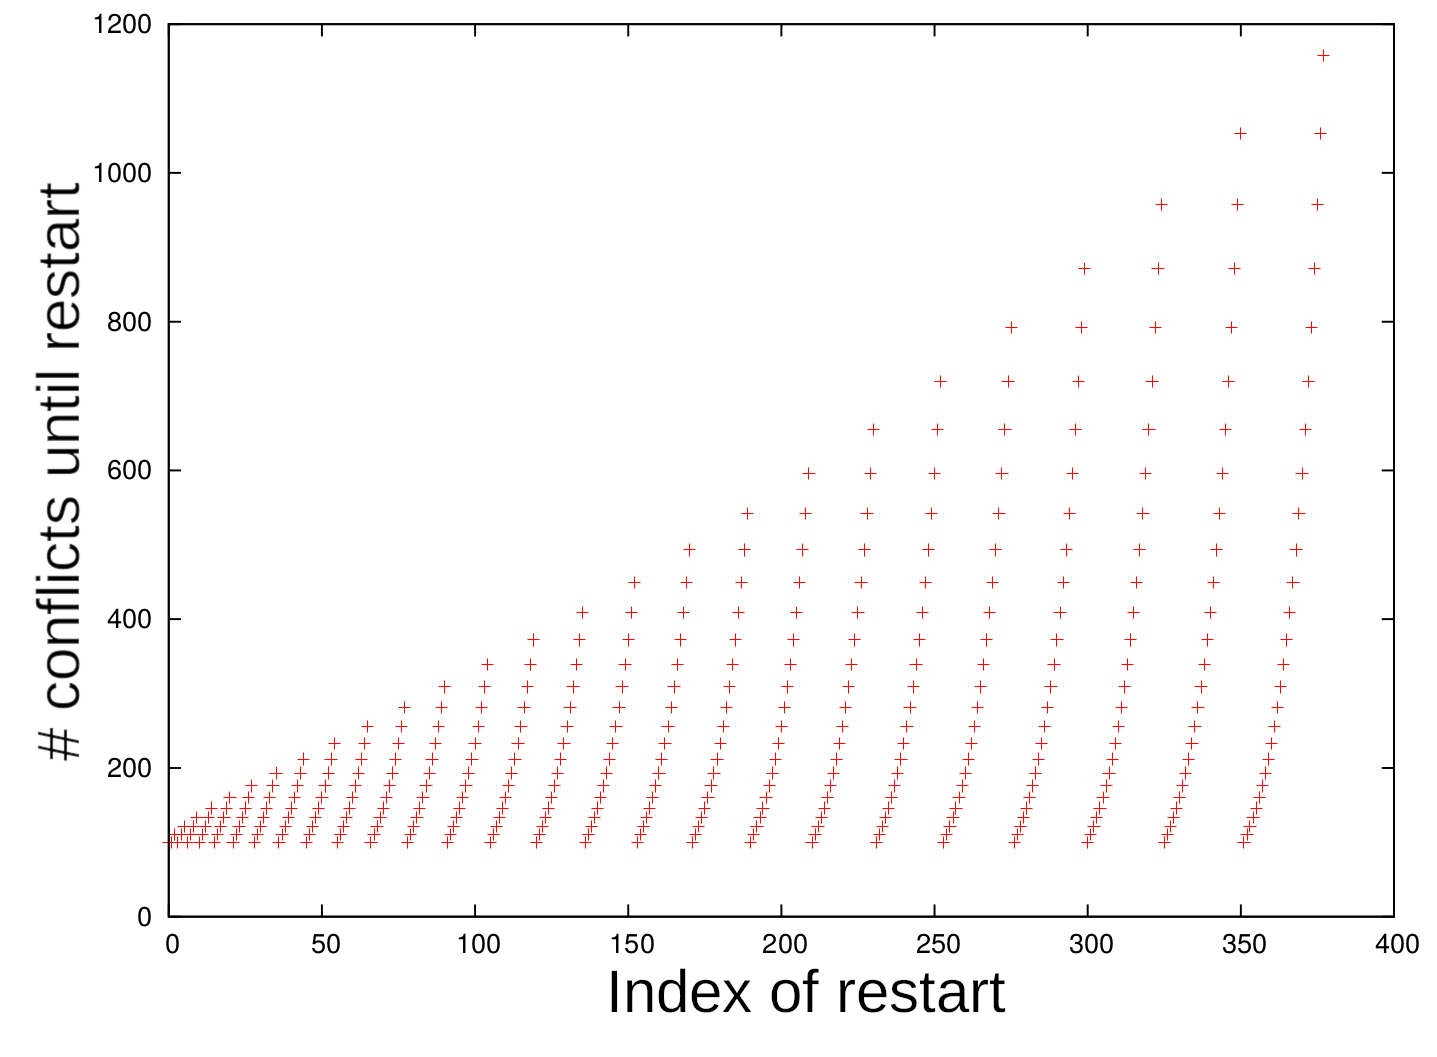
\includegraphics[width=\textwidth]{figures/l04/restart-inout-legend}
\end{column}
\begin{column}{0.45\textwidth}
\begin{algorithm}[H]
	\DontPrintSemicolon
	\caption{Inner / Outer}
	\KwData{int inner = 100, outer = 100}
	\BlankLine
	\While{true} {
		run DPLL() with conflict-limit $inner$\;
		restarts++\;
		\If{inner $\geq$ outer} {
			outer *= 1.1\;
			inner = 100\;
		}
		\Else{
			inner *= 1.1\;
		}
	}
\end{algorithm}
\end{column}
\end{columns}
\end{block}
\end{frame}

\begin{frame}{Restart Strategies: Luby Sequence}
\begin{theorem}[Luby, Sinclair, Zuckerman 1993]
	Consider a \highl{Las Vegas} algorithm $A$ (i.e., correct but with \highlo{random run time}) and a \highl{restart strategy} $S = \langle t_1, t_2, \ldots \rangle$ (i.e., run $A$ for time $t_1$, then for time $t_2$, etc.).	
	Up to a constant factor, the Luby sequence is the \highl{best possible universal strategy} to minimize the \highl{expected run time} until a run is successful.
	\begin{align*}
		Luby = u \cdot (t_i)_{i \in \mathbb{N}} \quad \text{with} \quad t_i = \begin{cases}
			2^{k-1} & \text{if $i = 2^k - 1$} \\
			t_{i-2^{k-1}+1} & \text{if $2^{k-1} \leq i \leq 2^k -1$} \\
		\end{cases}
	\end{align*}
\end{theorem}
\begin{example}[Luby Sequence]
$1, 1, 2, 1, 1, 2, 4, 1, 1, 2, 1, 1, 2, 4, 8, \dots$
\end{example}
\end{frame}
		
\begin{frame}{Restart Strategies: Luby Sequence}
\begin{block}{Luby Sequence: Naive Implementation}
	\begin{columns}[T]
	\begin{column}{0.45\textwidth}
		\centering
		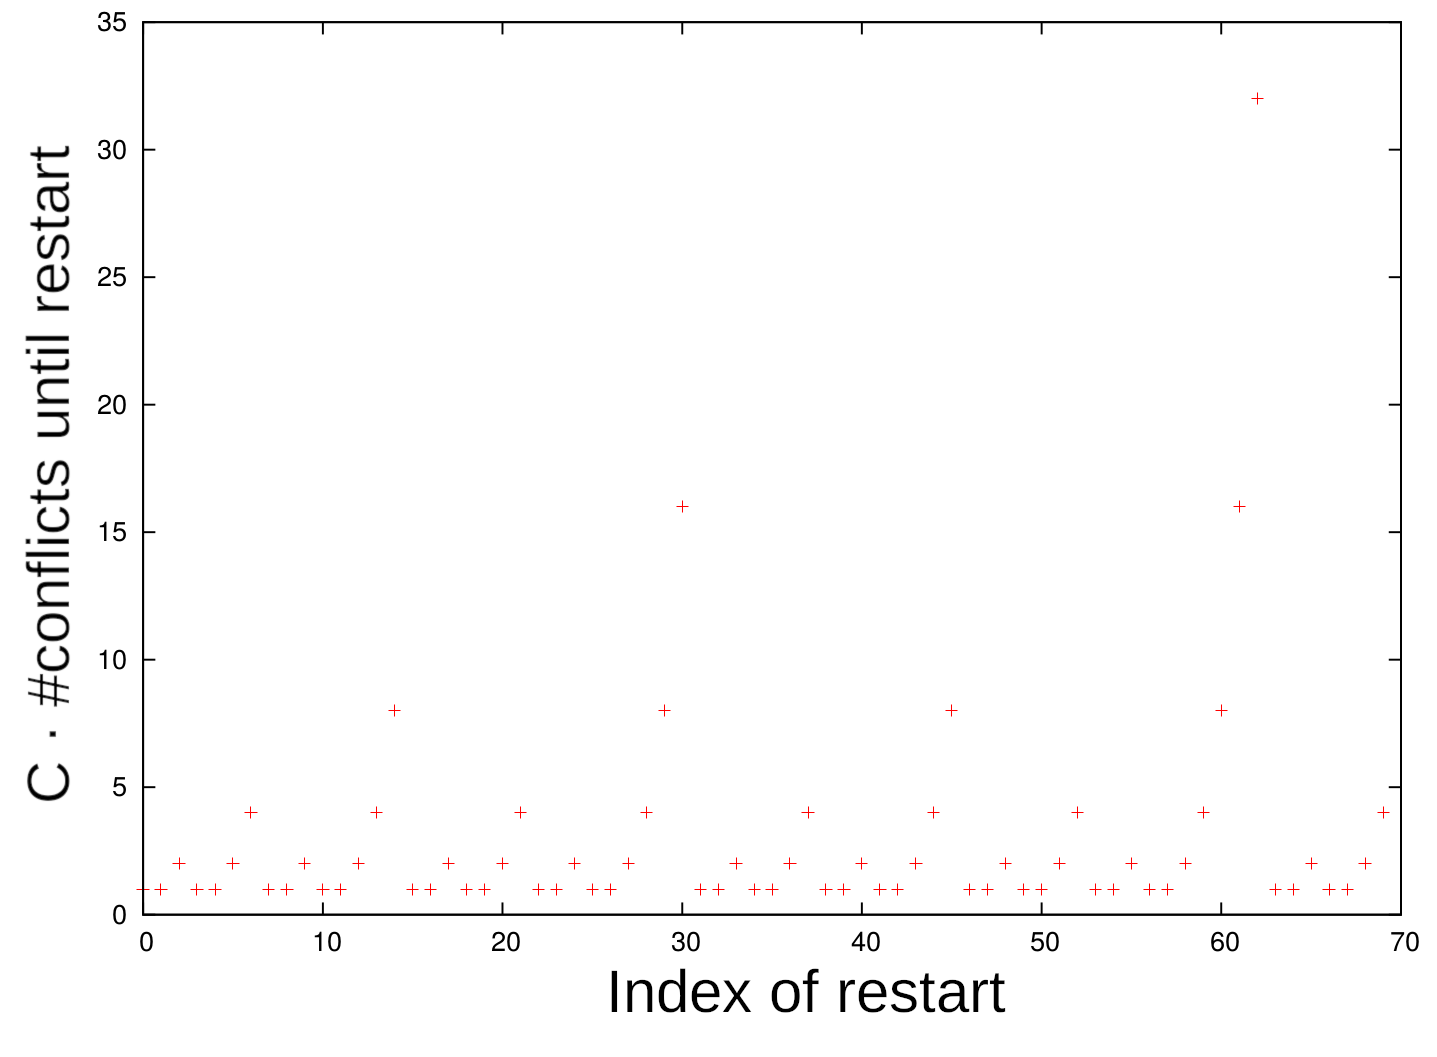
\includegraphics[width=\textwidth]{figures/l04/restart-luby-legend}
	\end{column}
	\begin{column}{0.5\textwidth}
	\begin{algorithm}[H]
		\DontPrintSemicolon
		\caption{Luby Sequence}
		\KwIn{int i}
		\BlankLine
		\For {$k = 1$ \KwTo $32$} {
			\If {$i == (1 \ll k) - 1$} {
				\Return $1 \ll (k-1)$
			}
		}
		\For {$k = 1$ \KwTo $\infty$} {
			\If {$(1 \ll (k-1)) \leq i \leq (1 \ll k) - 1$} {
				\Return Luby($i - (1 \ll (k-1)) + 1$)
			}
		}
	\end{algorithm}~\\[1ex]
	run DPLL() with conflict-limit $512 \cdot$ \text{Luby}(++restarts)
	\end{column}
	\end{columns}
\end{block}
\end{frame}
		
\begin{frame}{Restart Strategies: Luby Sequence}
\begin{block}{Luby Sequence: Reluctant Doubling}
A \highl{more efficient implementation} of the Luby sequence invented by Donald Knuth\\[1ex]
Use the $v_n$ of the following pairs $(u_n, v_n)$:\\[1ex]
a\texttt{($u_1$, $v_1$) = (1, 1);}\\
\texttt{($u_{n+1}$, $v_{n+1}$) = $u_n$ \& -$u_n$ == $v_n$\ ?\ ($u_n$+1, 1) :\ ($u_n$, 2$v_n$);}
\end{block}
\begin{example}[Luby Sequence]
(1,1), (2,1), (2,2), (3,1), (4,1), (4,2), (4,4), (5,1), \ldots
\end{example}
\end{frame}
		
\begin{frame}{Branching Polarity: Phase Saving}
Observation: Frequent {restarts} \highlo{decrease performance} on some satisfiable instances\\[1em]
\begin{block}{Assignment Caching}
Idea: Remember \highl{last assignment of each variable} and use it \highl{first} in branching
\begin{columns}[T]
\begin{column}{0.55\textwidth}
\begin{itemize}\setlength{\itemsep}{1em}
	\item First implemented in \href{http://reasoning.cs.ucla.edu/rsat/}{RSAT (2006)}
	\item Result: \highl{Phase saving} stabilizes positive effect of restarts
	\item Best results in combination with \highl{non-chronological backtracking}
\end{itemize}
\end{column}
\begin{column}{0.4\textwidth}
\centering
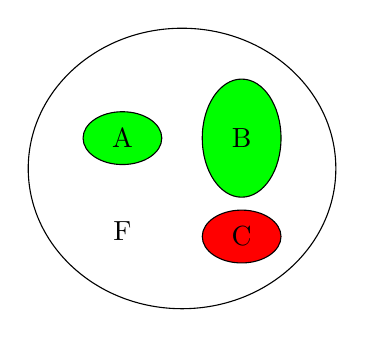
\begin{tikzpicture}[every node/.style = {draw, minimum width=1cm, minimum height=0.6cm}]
	\node (A) [ellipse, fill=green] {A};
	\node (B) [ellipse, fill=green, right=0.5cm of A, minimum width=1cm, minimum height=1.5cm] {B};
	\node (C) [ellipse, fill=red, below=0.15cm of B] {C\blitz};
	\node (D) [draw=none, ellipse, below=0.5cm of A] {F};
	\node (F) [ellipse, fit=(A) (B) (D)] {};
\end{tikzpicture}~\\
Example: $A$ and $B$ are satisfied, search works on component $C$
\end{column}
\end{columns}
\end{block}
\end{frame}

\begin{frame}{Recap}
	\begin{block}{Decision Heuristics}
	\end{block}
	\begin{block}{Restart Strategies}
		\begin{itemize}\setlength{\itemsep}{1ex}
			\item Inner / Outer Pattern
			\item Luby Sequence / Reluctant Doubling
			\item Phase Saving / Assignment Caching
		\end{itemize}
	\end{block}
	\begin{block}{Next up}
		Clause Learning
	\end{block}
\end{frame}


\begin{frame}{DPLL: Backtracking}

\begin{exampleblock}{Example: Chronological Backtracking}

\begin{minipage}{0.6\textwidth} 
\begin{tikzpicture}[node distance=2em]
\begin{scope}[node distance=2em]
\node at (current page.north east) (a) { A };
\node[below left=of a] (b0) { B };
\node[below right=of a] (b1) { [B=1] };
\end{scope}

\begin{scope}[node distance=3em]
\node[below left=of b0] (c0) { C };
\node[below right=of b0] (c1) { [C=1] };
\node[below left=of c0, xshift=1em] (x0) { X };
\node[below right=of c0, xshift=-1em] (x1) { X };
\node[below=of c1, yshift=1em] (x2) { X };
\end{scope}


\begin{scope}[node distance=1em]
\node[below left=of x0, xshift=1em, yshift=-1em] (y0) { [Y=1] };
\node[below right=of x0, xshift=-1em, yshift=-1em] (z0) { [Z]\blitz };
\node[below=of y0] (z1) { [Z]\blitz };

\node[below left=of x1, xshift=1em, yshift=-1em] (l0) {\blitz};
\node[below right=of x1, xshift=-1em, yshift=-1em] (l1) {\blitz};
\node[below left=of x2, xshift=1em, yshift=-1em] (l2) {\blitz};
\node[below right=of x2, xshift=-1em, yshift=-1em] (l3) {\blitz};
\end{scope}

\begin{scope}[every node/.append style = {font=\footnotesize, inner sep=2pt}]
\draw[->] (a) -- (b0) node [near start, left] {1};
\draw[->] (b0) -- (c0) node [near start, left] {1};
\draw[->] (c0) -- (x0) node [near start, left] {1};
\draw[->] (x0) -- (y0) node [near start, left] {1};
\draw[->] (y0) -- (z1) node [near start, left] {1};

\draw[->] (x0) -- (z0) node [near start, right] {0};

\draw[->] (a) -- (b1) node [near start, right] {0};
\draw[->] (b0) -- (c1) node [near start, right] {0};
\draw[->] (c0) -- (x1) node [near start, right] {0};
\draw[->] (c1) -- (x2) node [near start, right] {0};

\draw[->] (x1) -- (l0) node [near start, left] {1};
\draw[->] (x1) -- (l1) node [near start, right] {0};
\draw[->] (x2) -- (l2) node [near start, left] {1};
\draw[->] (x2) -- (l3) node [near start, right] {0};
\end{scope}

\only<1> {
\draw[->, myblue, line width=1.2pt] (a) -- (b0);
\draw[->, myblue, line width=1.2pt] (b0) -- (c0);
\draw[->, myblue, line width=1.2pt] (c0) -- (x0);
\draw[->, myblue, line width=1.2pt] (x0) -- (y0);
\draw[->, myblue, line width=1.2pt] (y0) -- (z1);
}
\only<2> {
\draw[->, myblue, line width=1.2pt] (a) -- (b0);
\draw[->, myblue, line width=1.2pt] (b0) -- (c0);
\draw[->, myblue, line width=1.2pt] (c0) -- (x0);
\draw[->, myblue, line width=1.2pt] (x0) -- (z0);
}
\end{tikzpicture}
\end{minipage}%
\begin{minipage}{0.39\textwidth} 
~\\[-3em]
\begin{align*}
F = \bigl\{ & \{A, B\}, \\
& \{B, C\}, \\
& \{\neg A, \neg X, Y \}, \\
& \{\neg A, X, Z\}, \\
& \{\neg A, \neg Y, Z\}, \\
& \{\neg A, X, \neg Z\}, \\
& \{\neg A, \neg Y, \neg Z \} \bigr\}
\end{align*}

\begin{itemize}
\item Trail: 
\only<1>{$A, B, C, X, Y, Z$}
\only<2>{$A, B, C, \neg X, Z$}
\item Conflicting Clause: 
\only<1>{\color{myred} $\{\neg A, \neg Y, \neg Z \}$}
\only<2>{\color{myred} $\{\neg A, X, \neg Z\}$}
\end{itemize}
\end{minipage}
\end{exampleblock}
\end{frame}


\begin{frame}{DPLL: Backtracking}
\begin{exampleblock}{Example: Backjumping}
\begin{minipage}{0.4\textwidth} 
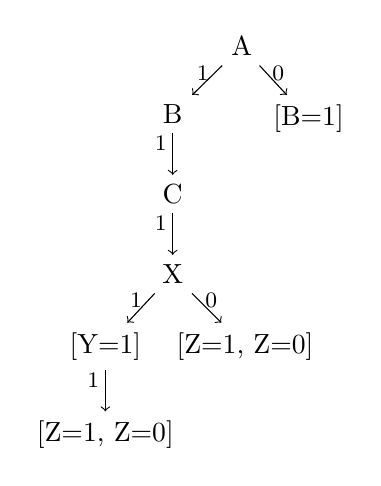
\begin{tikzpicture}[node distance=2em]
\begin{scope}[node distance=1.5em]
\node at (current page.north east) (a) { A };
\node[below left=of a] (b0) { B };
\node[below right=of a, xshift=-1em] (b1) { [B=1] };

\node[below=of b0] (c0) { C };
\node[below=of c0] (x0) { X };

\node[below left=of x0, xshift=1em] (y0) { [Y=1] };
\node[below right=of x0, xshift=-2em] (z0) { [Z=1, Z=0]\blitz };
\node[below=of y0] (z1) { [Z=1, Z=0]\blitz };
\end{scope}

\begin{scope}[every node/.append style = {font=\footnotesize, inner sep=2pt}]
\draw[->] (a) -- (b0) node [near start, left] {1};
\draw[->] (b0) -- (c0) node [near start, left] {1};
\draw[->] (c0) -- (x0) node [near start, left] {1};
\draw[->] (x0) -- (y0) node [near start, left] {1};
\draw[->] (y0) -- (z1) node [near start, left] {1};

\draw[->] (x0) -- (z0) node [near start, right] {0};

\draw[->] (a) -- (b1) node [near start, right] {0};
\end{scope}
\end{tikzpicture}


\end{minipage}%
\begin{minipage}{0.6\textwidth} 
\begin{itemize}
\item The first two conflicting clauses $\{\neg A, \neg Y, \neg Z \}$, $\{\neg A, X, \neg Z\}$ contain only a fraction of the assignments on the trail
\item Assignments to $B$ and $C$ obviously play no role in the present conflicting state and we could immediately backtrack to flip the assignment to $A$
\item How to find out which assignments on the trail are relevant for the actual conflict?
\end{itemize}
\end{minipage}
\end{exampleblock}
\end{frame}


\begin{frame}{Implication Graph}
Given: Formula $F$, assignment trail $T$ and conflicting clause $C$.

The implication graph is a DAG $G=(V \cup \{ \text{\blitz} \},E)$ of 
\begin{itemize}
	\item vertex \blitz representing the conflicting assignment (all literals of $C$ have edges to \blitz)
	\item vertices $v := [x=b,d]$ for each assignment $x=b$ (with decision level $d$)
	\item edges $e := ([l_i=0, d_i], [u=1, d_i])$ for each unit propagation of a literal $u$ from $[l_i=0, d_i]$ (due to a clause $\{ l_1,\dots, l_k, u \})$
\end{itemize}
\end{frame}


\begin{frame}{Conflict Analysis}
\only<1>{
The graph shows the implication graph for the conflicting state under the trail $A, B, C, X, Y, Z$. The edge labels denote clauses, node labels indicate an assignment and its decision level. 
}
\only<2>{
\begin{itemize}
\item the sink is always the conflicting assignment
\item the sources are the desicion literals that take part in the conflict
\item we can use it to detect the \emph{reasons} for a conflict
\end{itemize}
}
\only<3>{
In our example we can learn the clause $\{\neg A, \neg X\}$ in order to prevent the solver to pick the same partial assignment again. 
This can also be expressed as a sequence of resolution steps: $C = (7 \circ_Z 5) \circ_Y 3$
}
\begin{exampleblock}{Example: Implication Graph}
\vspace*{-1em}
\begin{minipage}{0.6\textwidth} 
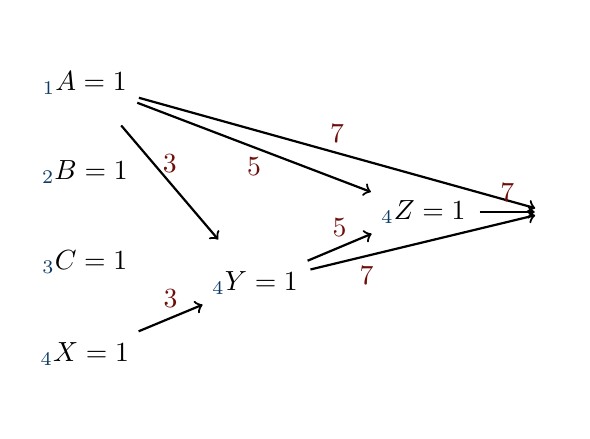
\begin{tikzpicture}[->, thick, node distance=0.7cm]
\node (A) [circle] { $_{\color{myblue} 1}A=1$ };
\node (B) [circle, below=of A, yshift=1cm] { $_{\color{myblue} 2}B=1$ }; 
\node (C) [circle, below=of B, yshift=1cm] { $_{\color{myblue} 3}C=1$ };
\node (X) [circle, below=of C, yshift=1cm] { $_{\color{myblue} 4}X=1$ };
\node (Y) [circle, right=of X, yshift=0.9cm] { $_{\color{myblue} 4}Y=1$ };
\node (Z) [circle, right=of Y, yshift=0.9cm] { $_{\color{myblue} 4}Z=1$ };
\node (empty) [circle, right=of Z] { \blitz };

\draw (A) -- (Y) node [midway, above] {\color{myred} 3 };
\draw (A) -- (Z) node [midway, below] {\color{myred} 5 };
\draw (A) -- (empty) node [midway, above] {\color{myred} 7 };
\draw (Y) -- (Z) node [midway, above] {\color{myred} 5 };
\draw (Z) -- (empty) node [midway, above] {\color{myred} 7 };
\draw (X) -- (Y) node [midway, above] {\color{myred} 3 };
\draw (Y) -- (empty) node [near start, below] {\color{myred} 7 };
\end{tikzpicture}
\end{minipage}%
\begin{minipage}{0.4\textwidth} 
\begin{align*}
F = \{ & \{A, B\}, & =:{\color{myred}1}\\
& \{B, C\}, & =:{\color{myred}2}\\
& \{\neg A, \neg X, Y \}, & =:{\color{myred}3}\\
& \{\neg A, X, Z\}, & =:{\color{myred}4}\\
& \{\neg A, \neg Y, Z\}, & =:{\color{myred}5}\\
& \{\neg A, X, \neg Z\}, & =:{\color{myred}6}\\
& \{\neg A, \neg Y, \neg Z \} \}& =:{\color{myred}7}
\end{align*}
\end{minipage}
\end{exampleblock}
\end{frame}
			
			
\begin{frame}{Implementation: Conflict Analysis}
\begin{itemize}
\item for each assignment store a pointer to the \emph{reason clause} and the \emph{decision level} on a stack
\item decision literals store a null pointer
\item with the clause pointers and the trail we can trace all the implications back to their sources
\end{itemize}
\begin{exampleblock}{Example: Trail with conflicting clause $\{\lnot A, \lnot Y, \lnot Z \}$}
\begin{tabular}{ccl}
\blitz & 4 & $\{\lnot A, \lnot Y, \lnot Z \}$ \\
Z & 4 & $\{\lnot A, \lnot Y, Z \}$ \\
Y & 4 & $\{\lnot A, \lnot X, Y \}$ \\
X & 4 & null\\
C & 3 & null\\
B & 2 & null\\
A & 1 & null\\
\end{tabular}
\end{exampleblock}
\end{frame}


\begin{frame}{Implementation: Conflict Analysis}
\begin{exampleblock}{Example: Trail with conflicting clause $\{\lnot A, \lnot Y, \lnot Z \}$}
\begin{minipage}{.37\linewidth}
\begin{tabular}{ccl}
\blitz & 4 & $\{\lnot A, \lnot Y, \lnot Z \}$ \\
Z & 4 & $\{\lnot A, \lnot Y, Z \}$ \\
Y & 4 & $\{\lnot A, \lnot X, Y \}$ \\
X & 4 & null\\
C & 3 & null\\
B & 2 & null\\
A & 1 & null\\
\end{tabular}
\end{minipage}%
\begin{minipage}{.65\linewidth}
\vspace*{-2em}
\textbf{Trail Resolution:}
\setlength{\leftmargini}{1em}
\begin{itemize}
\item $\{\lnot A, \lnot Y, \lnot Z\}\!\otimes_Z\!\{\lnot A, \lnot Y, Z\}\!=\!\{\lnot A, \lnot Y\}$
\item $\{\lnot A, \lnot Y\}\!\otimes_Y\!\{\lnot A, \lnot X, Y \}\!=\!\{\lnot A, \lnot X\}$
\item Conflict Clause $C = \{\lnot A, \lnot X\}$
\item Backtrack Level $b = 1$
\end{itemize} 
\end{minipage}
\end{exampleblock}

\begin{block}{Properties of conflict clause C}
\begin{itemize}
\item $F \models C$ 
\item $F \cup \lnot C \vdash_{UP} \bot$
\item $D \notin F, \forall D \subseteq C$
\end{itemize}
\end{block}
\end{frame}


\begin{frame}{Unit Implication Points (UIP)}
\begin{itemize}
	\item UIP is a dominator in the implication graph
	\item A node $v$ is a dominator for \blitz, if all paths to \blitz contain $v$
	\item FirstUIP: ``first'' dominator (seen from conflict side)
\end{itemize}

\begin{exampleblock}{Several possibilities to learn a clause from an implication graph}
A clause can be learned for every cut in the the implication graph.\footnote{Understanding the Power of Clause Learning (2003, Beame et al.)}%
\begin{center}%
~\\[-2em]
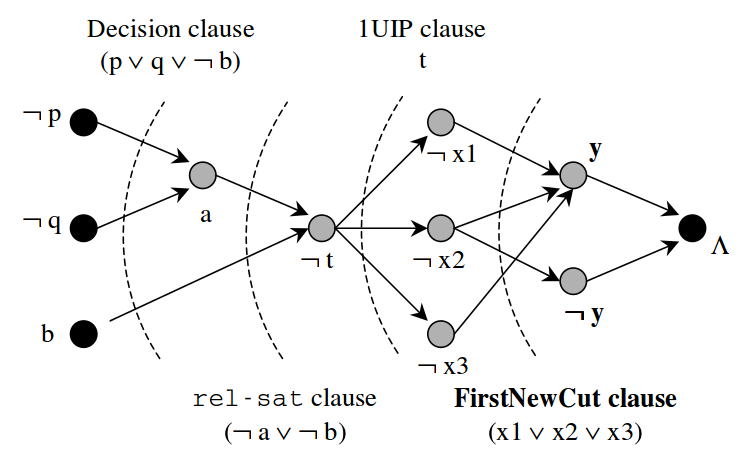
\includegraphics[width=.5\linewidth]{figures/l04/implicationgraphcuts.png}
\end{center}
\end{exampleblock}%
\end{frame}
			
			
\begin{frame}{Unit Implication Points (UIP)}
\begin{block}{1-UIP Learning}
\begin{itemize}
\item FirstUIP-clause: resolve conflicting clause and reason clauses until only a single literal of the current decision level remains 
\item Advantage: Stopping at a UIP always leads to an asserting clause. Algorithm becomes easier: backtrack until clause becomes asserting
\item The assertion level is the second highest level in a conflict clause
\end{itemize}
\end{block}
\end{frame}


\begin{frame}{Backtracking with Clause Learning}
1-UIP learning changes the decision tree in our example like this:

\begin{exampleblock}{Example: Non-chronological Backtracking}
\begin{minipage}{0.4\textwidth} 
\begin{tikzpicture}[node distance=2em]
\begin{scope}[node distance=1.5em]
\node at (current page.north east) (a) { A };
\node[below left=of a, xshift=-2em] (b0) { B };
\node[below right=of a, xshift=2em] (b1) { [B=1] };

\node[below=of b0] (c0) { C };
\node[below=of c0] (x0) { X };

\node[below=of x0] (y0) { [Y=1] };
\node[below=of y0] (z1) { [Z=1, Z=0]\blitz };

\node[below=of a] (y1) { [Y=0]};
\node[below=of y1] (x1) { [X=0]};
\node[below=of x1] (z0) { [Z=1, Z=0]\blitz };
\end{scope}

\begin{scope}[every node/.append style = {font=\footnotesize, inner sep=2pt}]
\draw[->] (a) -- (b0) node [near start, left] {1~~};
\draw[->] (b0) -- (c0) node [near start, left] {1};
\draw[->] (c0) -- (x0) node [near start, left] {1};
\draw[->] (x0) -- (y0) node [near start, left] {1};
\draw[->] (y0) -- (z1) node [near start, left] {1};

\draw[->] (a) -- (y1) node [near start, left] {1};
\draw[->] (y1) -- (x1);
\draw[->] (x1) -- (z0);

\draw[->] (a) -- (b1) node [near start, right] {~~0};

\only<1> {
\draw[->, myblue, line width=1.2pt] (a) -- (b0);
\draw[->, myblue, line width=1.2pt] (b0) -- (c0);
\draw[->, myblue, line width=1.2pt] (c0) -- (x0);
\draw[->, myblue, line width=1.2pt] (x0) -- (y0);
\draw[->, myblue, line width=1.2pt] (y0) -- (z1);
}
\only<2> {
\draw[->, myblue, line width=1.2pt] (a) -- (y1);
\draw[->, myblue, line width=1.2pt] (y1) -- (x1);
\draw[->, myblue, line width=1.2pt] (x1) -- (z0);
}
\end{scope}
\end{tikzpicture}
\end{minipage}%
\begin{minipage}{0.6\textwidth} 
\begin{align*}
F = \{ & \{A, B\}, \{B, C\}, \\
& \{\neg A, \neg X, Y \}, \\
& \{\neg A, X, Z\}, \\
& \{\neg A, \neg Y, Z\}, \\
& \{\neg A, X, \neg Z\}, \\
& \{\neg A, \neg Y, \neg Z \}%
\only<2>{\\ & {\color{myred} \{\neg A, \neg Y \} }} %
\}
\end{align*}%
Trail: 
\only<1>{$A, B, C, X, Y, Z$}
\only<2>{$A, \neg Y, \neg X, Z$}
\\
Conflicting Clause: 
\only<1>{\color{myred} $\{\neg A, \neg Y, \neg Z \}$}
\only<2>{{\color{myred} $\{\neg A, X, \neg Z\}$}}
{\only<1>{\\ {\color{black} Conflict Clause (1UIP): }{\color{myred} $\{\neg A, \neg Y \}$ }}}
\end{minipage}
\end{exampleblock}
\end{frame}
			
\begin{frame}{Resolution Proof}
\begin{block}{CDCL can derive a complete resolution refutation}
\begin{itemize}
\item proof can serve as a certificate for validating the correctness of the SAT solver\footnote{\url{http://www.cs.utexas.edu/~marijn/drat-trim/}}
\item resolution refutations based on clause learning find key practical applications (e.g. model checking) 
\item can help to determine minimally unsatisfiable subsets in an unsatisfiable formula
\end{itemize}
\end{block}
\end{frame}

			

\end{document}
